\section{Representative Examples}
Given the theoretical framework for downfolding a many orbital (or many-electron) problem to a 
few orbital (or few-electron) problem, we now discuss examples which elucidate the DMD method. 
The examples are as follows:
\begin{itemize}
\item Section~\ref{subsection:3band}: Three-band Hubbard $\rightarrow$ one-band Hubbard at half filling. Demonstrates finding a basis set for the second quantized operators and uses a set of eigenstates directly sampled from the low-energy space to find a one-band model.
\item Section~\ref{subsection:1dhydrogen}: Hydrogen chain $\rightarrow$ one-band Hubbard model at half filling. Demonstrates basis sets for {\it ab-initio} systems and the possibility to use this technique to determine the quality of a model to a given physical situation.
\item Section~\ref{subsection:graphene}: Graphene $\rightarrow$ one-band Hubbard model with and without $\sigma$ electrons. Demonstrates using the downfolding procedure to examine the effects of screening due to core electrons. 
\item Section~\ref{subsection:fese}: FeSe molecule $\rightarrow$ $3d,4p,4s$ system. Demonstrates the use of matching pursuit to assess the importance of terms in an effective model and to select compact effective models.
\end{itemize}

In all examples we will highlight the important ingredients associated with DMD. First and foremost, is the choice 
of low energy space or energy window i.e. how our database of wavefunctions was generated. Associated with this is 
the choice of the one body space in terms of which the effective Hamiltonian is expressed. Finally, we discuss 
aspects of the functional forms or parameterizations that are expected to describe our physical 
problem. An important effective Hamiltonian that enters three out of our four representative examples is 
the single (or one-) band Hubbard model,
\begin{equation}
	H = -t \;\sum_{\langle i,j \rangle, \eta} \tilde{d}_{i,\eta}^{\dagger} \tilde{d}_{j,\eta} + U \;\sum_{i} \tilde{n}^{i}_{\uparrow} \tilde{n}^{i}_{\downarrow}\,,
\label{eq:oneband}
\end{equation}
where $t$ and $U$ are downfolded (renormalized) parameters, $\eta$ is a spin index, 
$\tilde{d}_{i,\eta}$ is the effective one-particle operator associated with spatial orbital (or site) $i$ 
and $n_{i,\eta}=\tilde{d}_{i,\eta}^{\dagger} \tilde{d}_{i,\eta}$ is the corresponding number operator.
$\langle i,j \rangle$ is used to denote nearest neighbor pairs.
A constant energy shift has been dropped from Eq.~\ref{eq:oneband}, but practically 
needs to be incorporated when carrying out DMD with total energies and 1-RDM and 2-RDM data. 

\subsection{Three-band Hubbard model to one-band Hubbard model at half filling}
\label{subsection:3band} 
Our first example is motivated by the high $T_c$ superconducting cuprates~\cite{Bednorz1986} that 
have parent Mott insulators with rich phase diagrams on electron or hole doping~\cite{Dagotto_RevModPhys, LeeWen_RevModPhys}. 
Many works have been devoted to their model Hamiltonians and corresponding parameter 
values~\cite{tJSpalek, Pavirini, Emery, ZhangRice, Hybertsen_PRB1989, Hybertsen_PRB1990, Kent_Hubbard}. 
The emergent consensus of the minimal model involving both the copper and oxygen degrees of freedom 
is the three-orbital or three-band Hubbard model, 
\begin{eqnarray}
H &=&    \epsilon_p \sum_{j,\eta} n^{p}_{j,\eta} + \epsilon_{d} \sum_{i,\eta}  n^{d}_{i,\eta} 
	+ t_{pd} \sum_{\langle i,j \rangle, \eta} \text{sgn}(p_i,d_j) \Big( d_{i,\eta}^{\dagger} p_{j,\eta} + \text{h.c.} \Big) \nonumber \\
  & &   + U_p \sum_{j} n^{p}_{j,\uparrow} n^{p}_{j,\downarrow} + U_d \sum_{i} n^{d}_{i,\uparrow} n^{d}_{i,\downarrow} + V_{pd} \sum_{\langle i,j \rangle} n^{j}_p n^{i}_d\,,
\end{eqnarray}
where $d_i,p_j$ refer to the  $d_{x^2 - y^2}$ orbitals of copper (at site $i$) and $p_x$ or $p_y$ 
oxygen (at site $j$)  respectively and $\text{sgn}(p_i,d_j)$ is the sign of the hopping $t_{pd}$ 
between nearest neighbors, shown schematically in Fig.~\ref{fig:threeband}. 
$\epsilon_d$ and $\epsilon_p$ are orbital energies, $U_d$ and $U_p$ are strengths of onsite Hubbard interactions,  
and $V_{pd}$ is the strength of the density-density interactions between a neighboring $p$ and $d$ orbital. 
We keep the exposition simple and consider only the case where $\epsilon_p$, $U_d$ and $t_{pd}$ 
are non zero; the latter is chosen throughout this section to be the typical value of $1.3$ eV to give the reader a sense of overall energy 
scales. Since we work with fixed number of particles we set our reference zero energy 
to be $\epsilon_d = 0$, thus the charge transfer energy $\Delta \equiv \epsilon_p - \epsilon_d$ equals $\epsilon_p$ in our notation. 
We work in the hole notation; half filling corresponds to two spin-up and two spin-down holes on the $2\times2$ cell.
%$\uparrow$ and 2$\downarrow$ holes on the $2\times2$ cell.

\begin{figure}
\centering

\includegraphics[width=0.8\linewidth]{./Figures/three_band_figure.eps}
\caption{Schematic for downfolding the three-band Hubbard model to the one-band Hubbard model. The oxygen orbitals are 
eliminated to give "dressed" $d$-like orbitals of the one-band model, with modified hopping and interaction parameters. 
The relationship between the $\tilde{d}$ and the copper and oxygen orbitals is encoded by a linear transformation 
${\bf T}$ which is parameterized by $\alpha_1$, $\alpha_2$, $\alpha_3$, $\alpha_4$ and $F$ (see text for more details).}
\label{fig:threeband} 
\end{figure}

It is our objective to determine what one-band Hubbard model~[Eq.~\eqref{eq:oneband}]
``best" describes the three-band data. The effective \textit{d-like} orbitals $\tilde{d}_{i,\eta}$, 
that enter the low energy description are mixtures of copper and oxygen orbitals; this optimal transformation also remains an unknown. 
Thus the model determination involves two aspects (1) what are the composite objects that give a 
compact description of the low energy physics? and (2) given this choice what are the effective interactions between them? 
(A similar problem was posed and solved by one of us in the context of spin systems~\cite{Changlani_percolation}.)
In addition, the "best" effective Hamiltonian description depends on the energy scale of interest. 
All these issues will be addressed in the remainder of the section. 

We begin by encoding the relationship between the bare and effective operators as a linear transformation ${\bf T}$, 
\begin{equation}
	\tilde{d}_{i,\eta} = \sum_{j} T_{ij} c_{j,\eta}
\label{eq:dc}
\end{equation}
where $c_{j,\eta}$ is the hole (destruction) operator and refers to either the bare $d$ or $p$ orbitals. 
Further generalizations of this relationship (for example, including higher body terms) are also possible, but have not been considered here. 
For the $2\times2$ unit cell, {\bf T} is a $4 \times 12 $ matrix, which we parameterize by four distinct 
parameters after accounting for the symmetries of the lattice. 
Using the numbering of the orbitals corresponding to Fig.~\ref{fig:threeband}, the explicit form of ${\bf T}$ is
\begin{eqnarray}
{\bf T} = 
\left(
\begin{array}{cccccccccccc}
F        & \alpha_2 &        \alpha_2 &  \alpha_4 & \alpha_1 & \alpha_1 & -\alpha_1 & -\alpha_1 & \alpha_3 & -\alpha_3 & \alpha_3 & -\alpha_3 \\
\alpha_2 &  F       &        \alpha_4 &  \alpha_2 & \alpha_3 & -\alpha_1 & \alpha_1 & -\alpha_3 & -\alpha_3 & \alpha_3 & \alpha_1 & -\alpha_1 \\
\alpha_2 & \alpha_4 & F               &  \alpha_2 & -\alpha_1 & \alpha_3 & -\alpha_3 & \alpha_1 & \alpha_1 & -\alpha_1 & -\alpha_3 & \alpha_3 \\
\alpha_4 & \alpha_2 & \alpha_2        &   F       & -\alpha_3 & -\alpha_3 & \alpha_3 & \alpha_3 & -\alpha_1 & \alpha_1 & -\alpha_1 & \alpha_1 \\
\end{array}
\right)\,,
\end{eqnarray}
where we have defined $F \equiv \sqrt{1-4{\alpha_1}^2 - 2{\alpha_2}^2 - 4 {\alpha_3}^2 -{\alpha_4}^2}$. 
The parameters $\alpha_1$, $\alpha_2$, $\alpha_3$ and $\alpha_4$ will be optimized to minimize a certain cost function, 
which will be explained shortly. 

All RDMs in the three-band and one-band descriptions are also related via ${\bf T}$; 
the ones that we focus on are evaluated in eigenstate $s$ and are given by,
\begin{subequations}
\begin{eqnarray}
	\langle {\tilde{d}_{i,\eta}}^{\dagger} \tilde{d}_{j,\eta} \rangle_{s} &=& \sum_{mn} T^{*}_{im} \langle {c_{m,\eta}}^{\dagger} c_{n,\eta} \rangle_{s} T_{jn} \label{eq:dmstransformations1} \,,\\
	\langle \tilde{n}_{i,\uparrow} \tilde{n}_{i,\downarrow} \rangle_{s} &=& \sum_{jkmn} T^{*}_{ij} T^{*}_{im} \langle {c_{j,\uparrow}}^{\dagger} {c_{m,\downarrow}}^{\dagger} c_{n,\downarrow} c_{k,\uparrow} \rangle_{s} T_{in} T_{ik}\,.
\label{eq:dmstransformations2}
\end{eqnarray}
\end{subequations}
We optimize ${\bf T}$ by demanding two conditions be satisfied, (1) the effective orbitals ($\tilde{d}_{i,\eta}$) 
are orthogonal to each other i.e. $\Big({\bf T} {\bf T}^{\dagger}\Big)_{mn} = \delta_{mn}$
and (2) the sum of all diagonal entries (trace) of the 1-RDM of the effective orbitals for all low energy eigenstates 
equals the number of electrons of a given spin i.e. $\sum_{i} \sum_{\eta} \langle {\tilde{d}_{i,\eta}}^{\dagger} \tilde{d}_{i,\eta} \rangle_{s} = N_{\eta}$. 
These conditions are enforced by minimizing a cost function,
\begin{equation}
C = \sum_{s} \sum_{\eta} \Big( \sum_{i} \langle \tilde{d}_{i,\eta}^{\dagger} \tilde{d}_{i,\eta} \rangle_{s} - N_{\eta} \Big)^{2} + \sum_{mn} ( \Big({\bf T} {\bf T}^{\dagger}\Big)_{mn} -\delta_{mn})^{2}\,.
\label{eq:C}
\end{equation} 
For the $2\times2$ cell, $N_{\uparrow}=N_{\downarrow}=2$ and $i=1,2,3,4$. 
%a 12 orbital problem is downfolded to a 4 orbital one. 
The number of states $s$ was varied from three to six, depending on the energy window of interest.  

Fig.~\ref{fig:varyUdep} shows regimes of the three-band model where 
the lowest six eigenstates are separated from the higher energy manifold; the 
fourth and fifth eigenstates are degenerate. 
In the large $U_d$ limit, charge fluctuations are suppressed and these six 
states correspond to the Hilbert space of $4 \choose 2$ states of the effective spin model in its $S_z=0$ sector.
These states have primarily \textit{d-like} character, an aspect we will verify in this section. 
The eigenstates outside of this manifold involve \textit{p-like} excitations which the one-band model is not designed 
to capture. 

To give a concrete and representative example of our results, we discuss the case of 
$U_d/t_{pd}=8$ and $\Delta/t_{pd}=3$. We chose the lowest three eigenstates 
of the three-band model for computing the cost in Eq.~\eqref{eq:C}. The 
optimal parameters of ${\bf T}$ were determined by a brute force scan in the four dimensional space of parameters 
with a linear grid spacing of $0.002$; yielding $\alpha_1=0.216$, $\alpha_2=0.042$, $\alpha_3=0.018$ and $\alpha_4=0.016$. 
The corresponding trace conditions and orthogonality are simultaneously %individually 
satisfied to a relative error within 0.5 percent, confirming the validity of Eq.~\eqref{eq:dc}. 
Importantly, the 1-RDM elements corresponding to nearest neighbors $\langle \tilde{d}_1^{\dagger} \tilde{d}_2 \rangle_s$ 
already provide estimates for $U/t$ of the effective model. 
For our test example, the absolute values of $\langle \tilde{d}_1^{\dagger} \tilde{d}_2 \rangle_s$ 
in states $s=1,2,3$ are approximately $0.159$, $0.142$ and $0.084$ respectively. 
Since the exact knowledge of the corresponding eigenstates of the one-band Hubbard model is directly available for arbitrary 
$U/t$ by exact diagonalization, we directly look up the $U/t$ with 
the same 1-RDM value. This matching procedure gives $(U/t)_1 \approx 14.1 $, $(U/t)_2 \approx 13.2 $, $(U/t)_3 \approx 12.7 $. 
Analogous estimates of $U/t$ were also made by comparing the 2-RDM elements $\langle \tilde{n}_{\uparrow} \tilde{n}_{\downarrow} \rangle_s$ 
with similar results. 

The state-matching approach was supported by DMD performed 
with the same three low-energy states, using their energies and 
the computed values of $\langle \tilde{d}_1^{\dagger} \tilde{d}_2 \rangle_s$ 
and $\langle \tilde{n}_{i,\uparrow} \tilde{n}_{i,\downarrow} \rangle_{s}$ from Eqs.~\eqref{eq:dmstransformations1} 
and~\eqref{eq:dmstransformations2}. 
(To mimic the situation characteristic of \textit{ab-initio} examples where no eigenstates are generally available, 
several non eigenstates were generated as random linear combinations of the lowest three eigenstates, with 
similar outcomes.) For our test example, we find $U/t = 13.45 $ and $t = 0.3025 $ eV, 
the former in the correct range of the state-matching values. (There is no error bar since there 
are three unknown parameters in the model Hamiltonian, including the constant energy shift, and there 
are three entries in the DMD procedure). As was expected, and observed, when the one-band description 
is good within a given window, all estimates of $U/t$ agree with each other. 
\begin{figure}
\centering
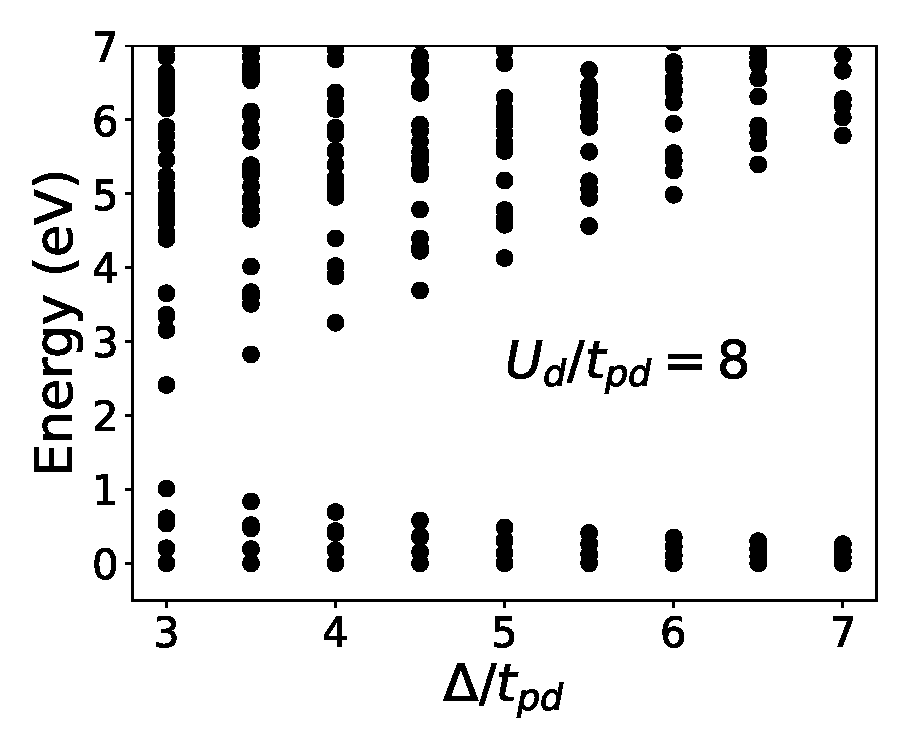
\includegraphics[width=0.45\linewidth]{./Figures/spectrum_vs_ep_Ud_8.eps}
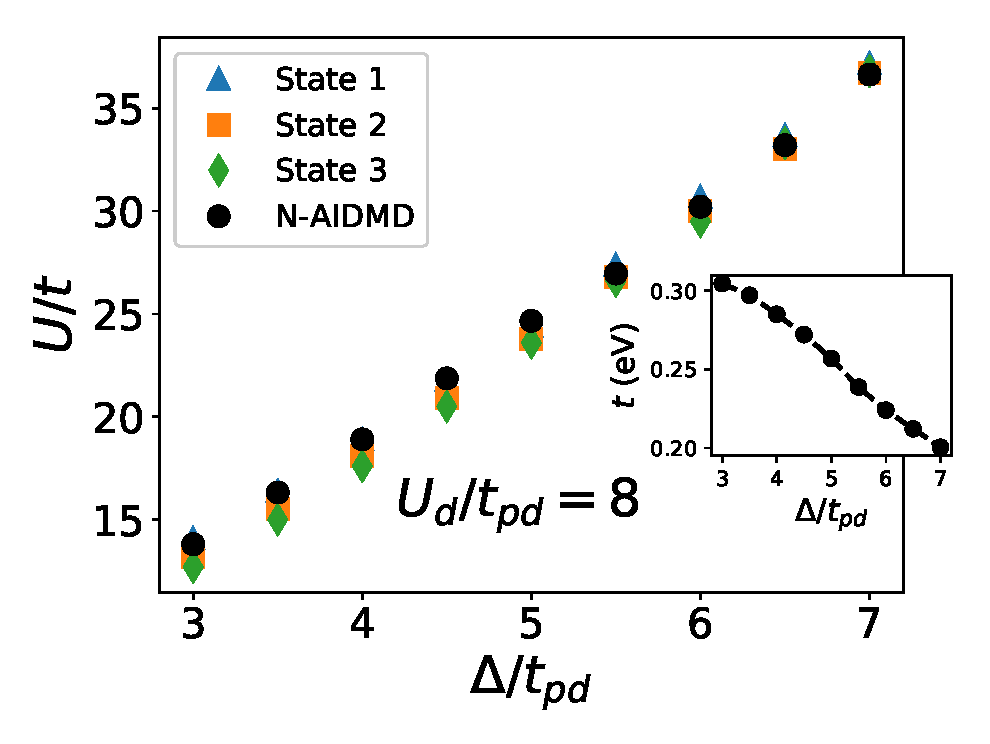
\includegraphics[width=0.49\linewidth]{./Figures/U_and_hopping_combined_vs_ep_Ud_8.eps}
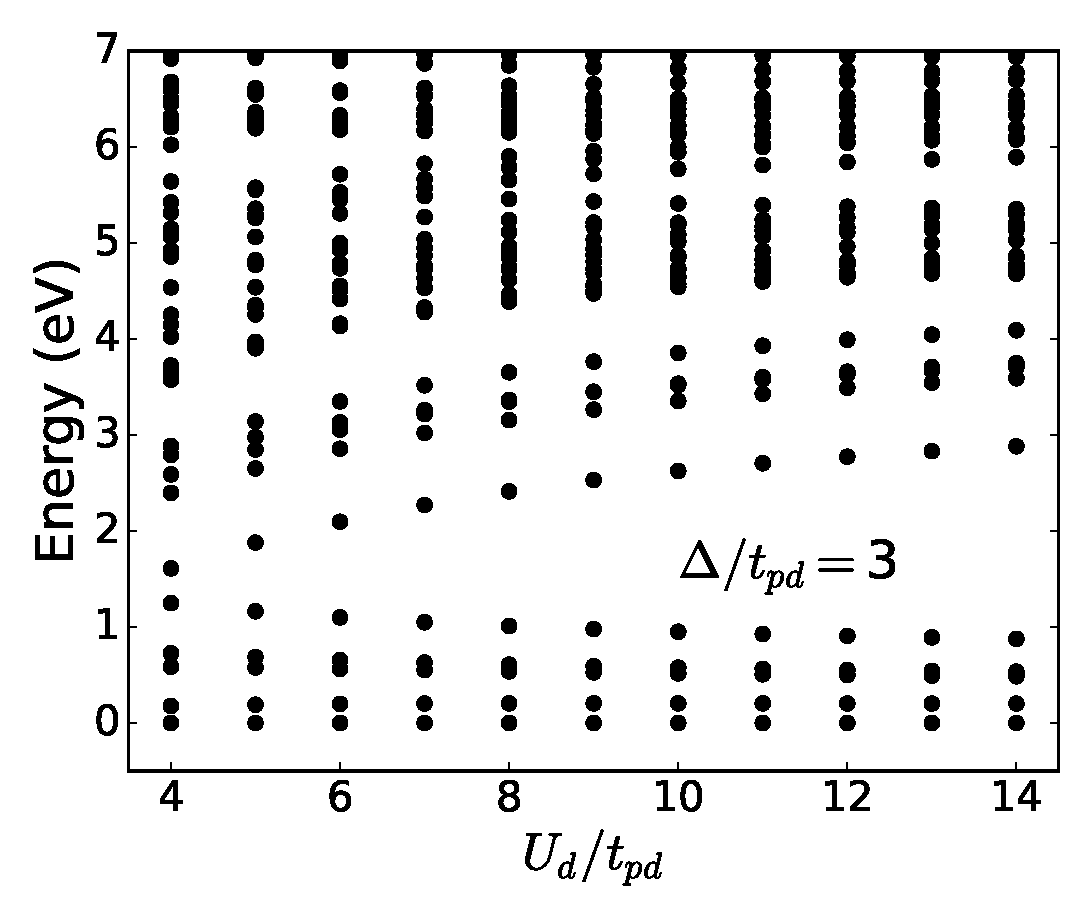
\includegraphics[width=0.45\linewidth]{./Figures/spectrum_vs_Ud_ep_3.eps}
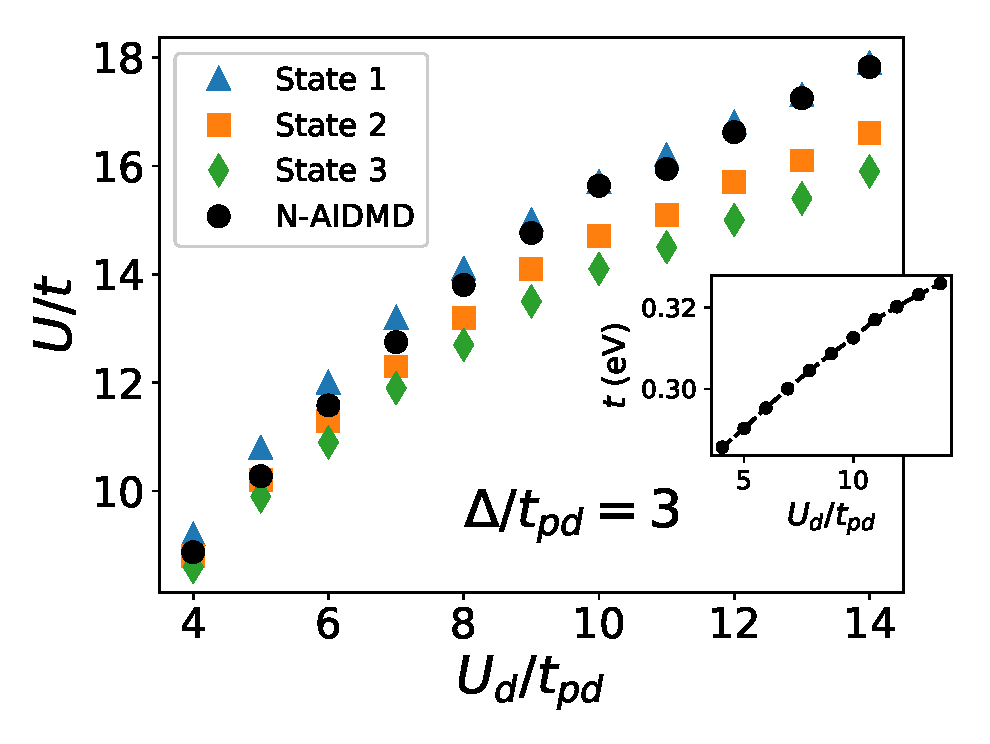
\includegraphics[width=0.48\linewidth]{./Figures/U_and_hopping_combined_vs_Ud_ep_3.eps}
\caption{Low energy spectra (relative to the corresponding ground state) for $t_{pd}=1.3$ eV 
and downfolded parameters for various parameter regimes of the three-band Hubbard model. 
The one-band $U/t$ values were obtained by state matching or by the DMD procedure using 
the lowest three eigenstates. The insets show $t$ obtained from DMD. 
(A) and (B) show the case of fixed $U_d/t_{pd}=8$ and varying $\Delta/t_{pd}$ 
and (C) and (D) show the case of fixed $\Delta/t_{pd}=3$ and varying $U_d/t_{pd}$.}
\label{fig:varyUdep} 
\end{figure}

Some trends in the one-band description are explored in Figure~\ref{fig:varyUdep} 
by monitoring the downfolded parameters as a function of varying $\Delta/t_{pd}$ and $U_d/t_{pd}$. 
For example, when $U_d/t_{pd}=8$ is fixed and $\Delta/t_{pd}$ is increased, we find that 
the effective hopping $t$ decreases and $U/t$ increases. This is physically reasonable since an increasing difference in the 
single particle energies of the copper and oxygen orbitals makes it energetically unfavorable for holes 
to hop between the two orbitals. When $\Delta/t_{pd}=3$ is fixed and $U_d/t_{pd}$ is increased, $U/t$ increases. 
As one mechanism of avoiding the large $U_d$, the copper orbitals are forced to hybridize more with the oxygen ones; 
on the other hand, hole delocalization is suppressed in a bid to maintain mostly one hole per $\tilde{d}$ due to the larger 
$U/t$. The net result of these effects is that the $t$ also increases.%, albeit only marginally; a trend also observed in $\alpha_1$.

Since DMD uses only information from the full model (here, three-band model) or \textit{ab-initio} calculation, it is imperative that we 
perform other sanity checks on the accuracy of the downfolded model. An important check for the one-band model is its 
ability to reproduce the low energy gaps of the three-band model; these have been compared in 
Figure~\ref{fig:energyfit}. For the case of $\Delta/t_{pd}=3$, we observe that for all $U_d/t_{pd}$ 
the lowest three eigenstates were reproduced well. 
%with an increased error  for the fourth and fifth (degenerate) 
%states and the largest error ($\approx 0.1 $ eV) for the sixth eigenstate.
This model also reproduces the states outside of the DMD energy window, although with a slightly larger errors. 
% This last eigenstate is 
%well outside the energy window used in the DMD to obtain $t$ and $U$. 
Similar trends are seen for the case of $\Delta/t_{pd}=5$, 
with the noticeable difference being that the energy error of the highest state has reduced. 
This reflects that the Hubbard parameters obtained from DMD are, in general, dependent on the energy window of interest, a 
point which we will highlight shortly by investigating it systematically. 

\begin{figure}
\centering
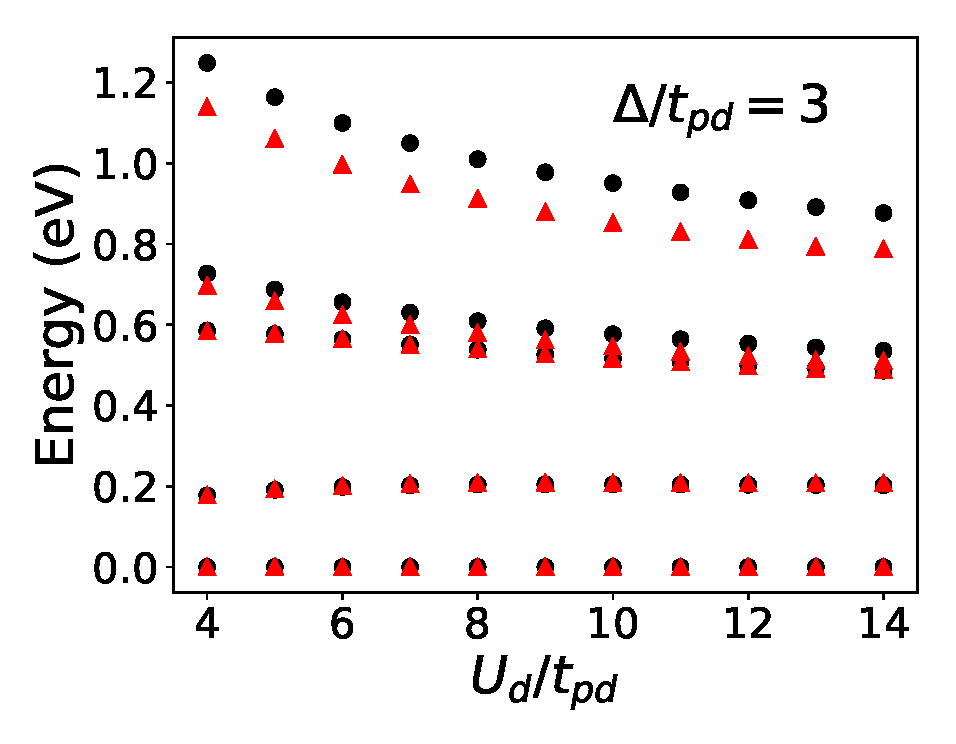
\includegraphics[width=0.49\linewidth]{./Figures/lowenergy_1and3_vs_Ud_ep_3.eps}
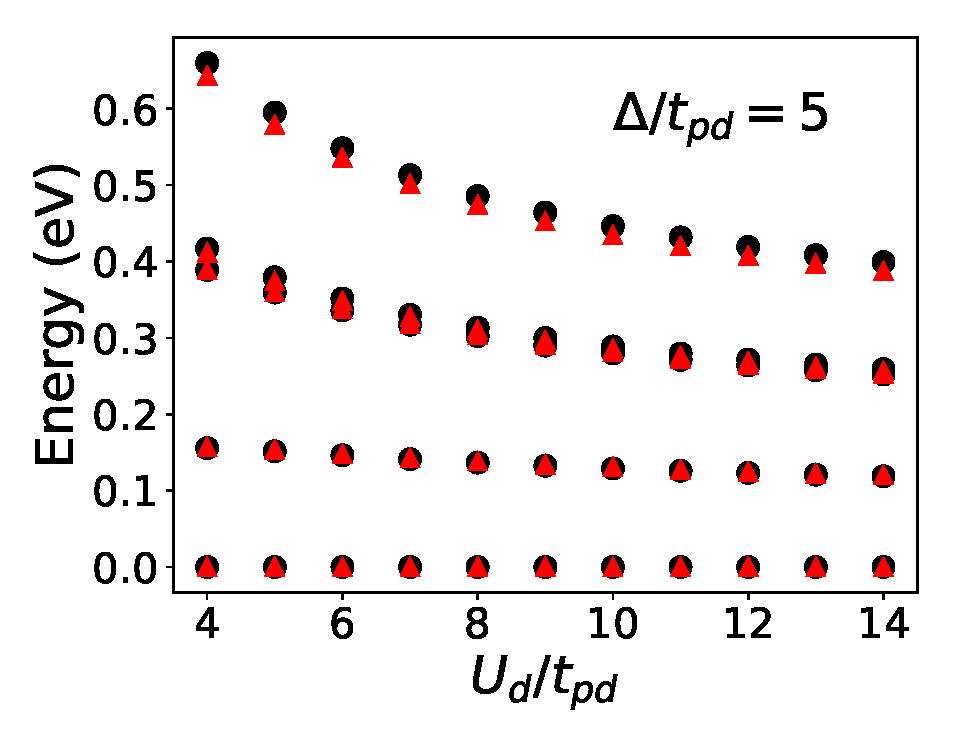
\includegraphics[width=0.49\linewidth]{./Figures/lowenergy_1and3_vs_Ud_ep_5.eps}
\caption{Comparison of energy gaps of the three-band (black circles) and downfolded 
one-band (red triangles) Hubbard models using the 
values of $U$ and $t$ for $t_{pd}=1.3$ eV and various $U_{d}/t_{pd}$ for 
fixed (A) $\Delta/t_{pd}=3$ and (B) $\Delta/t_{pd}=5$}
\label{fig:energyfit} 
\end{figure}	
Downfolding enables reduction of the size of the effective Hilbert space; allowing 
simulations of bigger unit cells to be carried out. To show that this actually works well in practice for the three-band case, 
we consider the $2\sqrt{2} \times 2 \sqrt{2}$ square unit cell, comprising of 8 copper and 16 oxygen orbitals. 
For representative test cases, we performed exact diagonalization calculations at half filling; 
the Hilbert space comprises of 112,911,876 basis states. Roughly 200 Lanczos iterations were carried out, 
enabling convergence of the lowest four energies. We compared the lowest gaps with the 
corresponding calculation on the single band model on the same square geometry, with a Hilbert space size of only 4900, 
using the downfolded parameters obtained from the smaller $2 \times 2$ cell. Our results are summarized 
in Table~\ref{tab:predictivity}. 

In all cases the agreement between the three-band and one-band models is remarkably good. 
The lowest energy gap error is within $0.0004$ eV (1\% relative error).%, which in relative terms was a maximum error of 1 percent. 
The largest error in the third gap is of the order of $0.005$ eV (3\% relative error). %which in relative terms is about 3 percent. 
These results indicate the reliability of the downfolding procedure 
and highlight its predictive power. 
This suggests that one could perform DMD on a small size system to obtain the effective model at a low cost. In the spirit of multiscale simulation, one could then solve this effective model (within its regime of validity) for larger systems at a significantly reduced cost compared to solving the original model or \textit{ab-initio} Hamiltonians.
%as long as one appreciates the limitations of the downfolded 
%model and its regime of validity.
Although, in more general situations, for example, models 
with long range interactions, finite size dependence of the downfolded parameters may also be important. 
Systematically understanding these cases is an endeavor we leave to future work. 
\begin{table}
\centering
\begin{tabular}{c|c|c|c||c|c||c|c||c|c}
\hline
$\Delta/t_{pd}$ & $U_d/t_{pd}$ & $t$ & $U/t$ & $G_{2-1,3}$ & $G_{2-1,1}$ & $G_{3-1,3}$ & $G_{3-1,1}$ & $G_{4-1,3}$ & $G_{4-1,1}$  \\
\hline
\hline
3.0 & 4.0 &  0.2839 & 8.698 & 0.0465 & 0.0461 & 0.1505 & 0.1489 & 0.2247 & 0.2201  \\ 
3.0 & 8.0 &  0.3025 & 13.45 & 0.0524 & 0.0528 & 0.1682 & 0.1681 & 0.2063 & 0.2020  \\ 
3.0 & 12.0 & 0.3155 & 16.58 & 0.0520 & 0.0524 & 0.1658 & 0.1649 & 0.1920 & 0.1866  \\ 
5.0 & 4.0 &  0.2326 & 15.08 & 0.0395 & 0.0398 & 0.1256 & 0.1258 & 0.1466 & 0.1458  \\ 
5.0 & 8.0 &  0.2501 & 23.75 & 0.0344 & 0.0347 & 0.1070 & 0.1070 & 0.1142 & 0.1138  \\ 
5.0 & 12.0 & 0.2647 & 29.89 & 0.0310 & 0.0312 & 0.0956 & 0.0955 & 0.0998 & 0.0993  \\ 
\hline
\end{tabular}
\caption{Comparison of low energy gaps of the 8 ($2\sqrt{2} \times 2\sqrt{2}$) unit cell 
at half filling for the one-band Hubbard (Hilbert space 4900) and three-band Hubbard (Hilbert space 112,911,876) 
models from exact diagonalizations, for six representative cases using $t_{pd}=1.3 $ eV. The notation $G_{i-j,m}$ 
has been used to indicate the gap (energy difference) between state $i$ and $j$ and $m=1,3$ is a label that 
refers to the 1- or three-band models. 
The downfolded parameters, $t$ and $U/t$, for the one-band model were those obtained from downfolding the 4 ($2\times2$) unit cell 
case.}
\label{tab:predictivity}
\end{table} 

Till this point, all our results focused on using only the lowest three eigenstates. We now explore 
the effect of increasing the energy window, by including higher eigenstates, using our 
test example of $U_d/t_{pd}=8$ and $\Delta/t_{pd}=3$. To do so, we now use 
all six low energy eigenstates for optimizing the cost function in Eq.~\ref{eq:C}. We 
find similar (but not exactly the same) values of $\alpha_i$ compared to 
the case when only the three lowest states were used. The fact that a low cost solution can be attained 
confirms our expectation that the entire low energy space of six states is consistently 
described by a set of $\tilde{d}_i$ operators. 
\begin{figure}
\centering
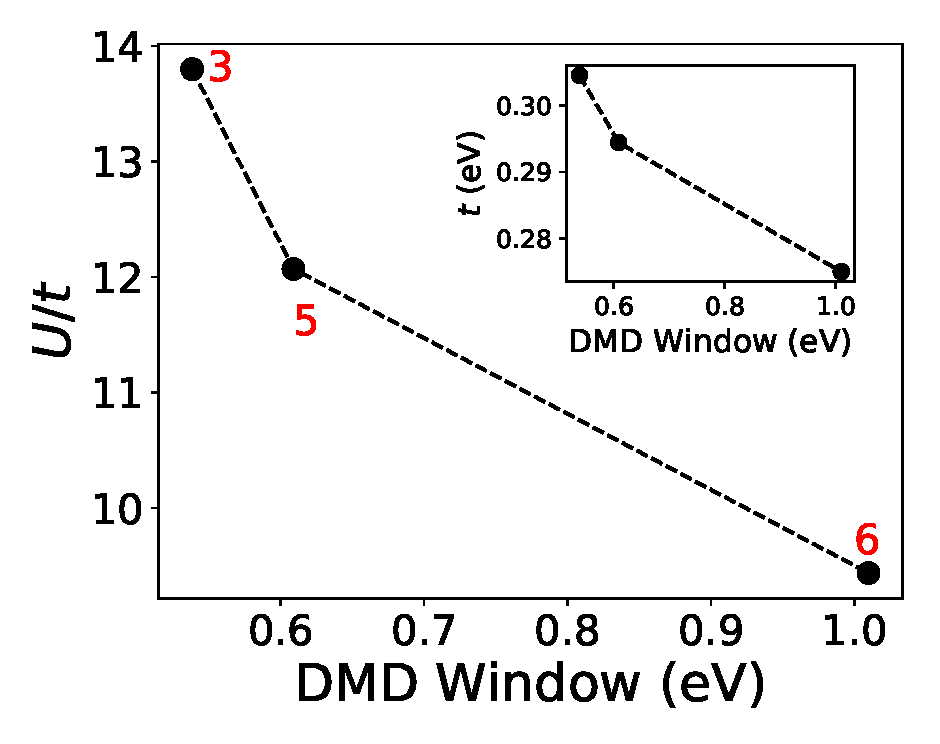
\includegraphics[width=0.49\linewidth]{./Figures/downfolded_params_diffwindows_ep_3.eps}
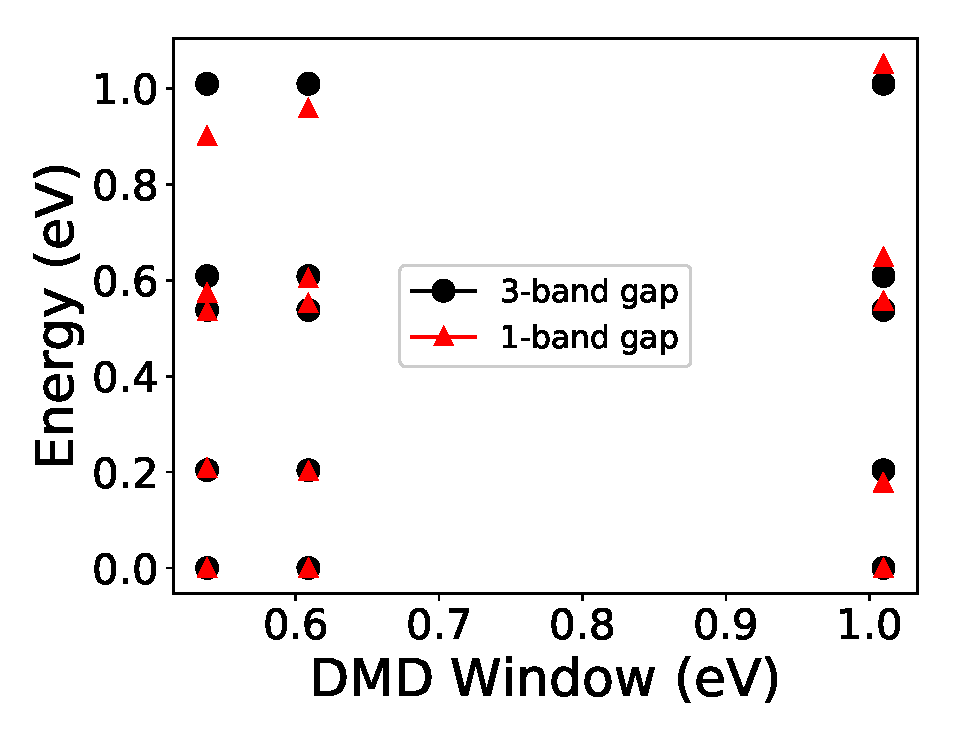
\includegraphics[width=0.49\linewidth]{./Figures/lowenergygaps_diffwindows_ep_3.eps}
\caption{All results are for $U_d/t_{pd}=8$ and $\Delta/t_{pd}=3$ and $t_{pd}=1.3$ eV 
(A) Downfolded values of $U/t$ and $t$ (inset) obtained by the DMD procedure using all eigenstates 
in a given energy window, increasing windows correspond to 3,5 and 6 low energy eigenstates. 
(B) Comparison of energy gaps between the three-band (black circles) and one-band (red triangles) 
Hubbard models for different energy windows using the downfolded values in that window.}
\label{fig:windows} 
\end{figure}	

However, as Fig.~\ref{fig:windows}(A) shows, the estimates of $U/t$ and $t$ depend on how many eigenstates 
are used in the DMD procedure. This is because the DMD aims to provide the one-band description 
that "best" describes \textit{all} states in a given window. If the model is not perfect within a given energy window, 
an energy dependent model is expected, consistent with the renormalization group perspective. For our test example, 
increasing the number of eigenstates from three to six changed $U/t$ from $13.8$ to $9.44$~\footnote{The attentive reader 
would have noticed the slightly different estimate of $U/t\approx 13.45$ when three states were used for both the DMD 
and cost minimization used to obtain effective orbitals. This is because the effective $\tilde{d}$ are 
slightly different in the two cases.} and $t$ from $0.3045$ to $0.2750$ eV. 
The features associated with the energy dependence are further confirmed in Fig.~\ref{fig:windows}(B). 
When only three states are used, the one-band (nearest neighbor) Hubbard model is insufficient for \textit{accurately}
describing states outside the window. When all six states are used, the DMD tries to minimize the error of the 
largest energy gap at the cost of errors in the smaller energy gaps. 
One could of course choose a different parameterization, say with additional next nearest neighbor $t'$, for which is 
may be possible to reduce this energy dependence significantly and thus have a model that describes the smaller 
and larger energy scales equally well.
 
 
